\documentclass[11pt]{article}
\usepackage{xcolor}
\usepackage{caption} 
\usepackage{graphicx}
\usepackage[italian]{babel}
\usepackage{natbib}
\usepackage[utf8]{inputenc}
\usepackage[a4paper,vmargin=30mm,hmargin=33mm,footskip=15mm]{geometry}
\usepackage{fancyhdr}
\usepackage{eurosym}
\renewcommand{\footrulewidth}{0.4pt}% default is 0pt
\rhead{
    \textbf{Document:} analisi requisiti |
    \textbf{Revision:} 0.2 \\
}
\setlength{\headheight}{25.2842pt}
\addtolength{\topmargin}{-13.2842pt}
\pagestyle{fancy}
\usepackage{hyperref}
\begin{document}

\begin{titlepage}
		\begin{center}
		    \Huge
			\textbf{JGuesser}
			
			\LARGE
			\vspace{0.85cm}
			Documento di progetto \\
            (Obiettivi e Requisiti)
			\vspace{0.5cm}
			
			
\includegraphics[scale=2.5]{images/logo_progetto_se-t24.png}
			
			\vfill
			
		    
\includegraphics[scale=0.200]{images/logo_unitn.png}
			
			\Large
			Dipartimento di Ingegneria e Scienza dell’Informazione \\
			Gruppo: T24 \\
			Membri: Lorenzo D'Ambrosio, Andrea Goldoni, Marco Murru
				
			\vspace{1.5cm}
    		
		\end{center}
	\end{titlepage}

\tableofcontents
\section*{Scopo del documento}
In questo documento sono spiegati gli obiettivi e i requisiti del progetto JGuesser. Più nello specifico verranno approfonditi: 
\begin{itemize}
    \item gli obiettivi del progetto;
    \item i requisiti funzionali e non funzionali;
    \item i requisiti del Front-End;
    \item i requisiti del Back-End.
\end{itemize}
\section{Obiettivi del progetto}
Il progetto ha come obiettivo la realizzazione di un applicazione web, che permetta di imparare gli alfabeti giapponesi, di tipo Hiragana, Katakana e Kanji. L’apprendimento degli alfabeti avviene attraverso il riconoscimento di particolari simboli giapponesi e l’identificazione del loro suono o significato. \\
\\
L’applicazione web si pone i seguenti obiettivi: 
\begin{enumerate}
    \item Dotare l’utente di un compendio degli alfabeti, necessario alla fruizione dell’applicazione web; \label{o1}
    
    \item Fornire all’utente una serie di quiz e sfide giornaliere per testare la propria conoscenza; \label{o2}
    
    \item Permettere agli utenti di registrarsi ed eventualmente acquistare un servizio premium, che darà l'accesso a funzionalità esclusive; \label{o3}
    
    \item Dare la possibilità agli utenti di affrontare altri giocatori attraverso sfide online; \label{o4}
    
    \item Permettere all’utente, di accedere ad una classifica mondiale; \label{o5}
    
    \item Permettere all'utente di accedere alla propria area personale, con statistiche e dati personali; \label{o6}
    
    \item Essere veloce e intuitiva, in modo da essere utilizzata sia da pc che da smartphone. \label{o7}
\end{enumerate}
\section{Requisiti Funzionali}
In questa sezione sono elencati i requisiti funzionali dell'applicazione, ovvero tutte quelle funzionalità che ci si aspetta che il sistema sia in grado di fornire. 
Ogni requisito sia funzionale, che non funzionale deve rispondere ad un obbiettivo.

\subsection{Compendio degli alfabeti} \label{req_compendio}
Attraverso un pulsante info, il sistema dà la possibilità all'utente di accedere alle seguenti informazioni:
\begin{itemize}
    \item breve descrizione degli alfabeti;
    \item tabella contenente tutti i simboli dell'alfabeto Hiragana;
    \item tabella contenente tutti i simboli dell'alfabeto Katakana;
    \item lista dei simboli dell'alfabeto Kanji.
\end{itemize}
Questa funzionalità è disponibile per tutti i tipi di utente. Questo requisito risponde all'obbiettivo \ref{o1}.

\subsection{Registrazione} \label{req_registrazione}
L'applicazione permetterà all'utente di creare un proprio account, per far ciò verrà richiesto all'utente di fornire i seguenti dati:
\begin{itemize}
    \item username, il quale dovrà essere univoco;
    \item e-mail, la quale dovrà essere univoca;
    \item password;
    \item nazione.
\end{itemize}
Inseriti i dati, prima di completare la registrazione l'utente dovrà cliccare sul reCAPTCHA, per dimostrare di essere un umano. Effettuata la registrazione verrà inviata all’utente un’e-mail di conferma dell’avvenuta registrazione. \\
Questa funzionalità è disponibile per i soli utenti guest. Questo requisito risponde all'obbiettivo \ref{o3}.

\subsection{Login con credenziali} \label{req_login_con credenziali}
Il sistema permetterà all'utente di accedere al proprio account, utilizzando le proprie credenziali. Questa funzionalità è disponibile per gli utenti registrati e di livello superiore. Questo requisito risponde all'obbiettivo \ref{o6}. 

\subsection{Login con google} \label{req_login_con_google}
Il sistema permetterà all'utente di accedere alla piattaforma utilizzando il proprio account google. In questo caso non verrà inviata alcuna e-mail, anche se l'utente sarà effettivamente registrato. \\
Questa funzionalità è disponibile per gli utenti non registrati. Questo requisito risponde all'obbiettivo \ref{o6}. 

\subsection{Logout} \label{req_logout}
Il sistema permetterà all'utente di uscire dal proprio account. Questa funzionalità è disponibile per gli utenti registrati e di livello superiore. Questo requisito risponde all'obbiettivo \ref{o6}. 

\subsection{Visualizzazione dati personali} \label{req_visualizzazione_dati_personali}
L'applicazione deve dare la possibilità all'utente di visualizzare i propri dati personali, inseriti in fase di registrazione, ovvero:
\begin{itemize}
    \item username;
    \item e-mail;
    \item password;
    \item nazione.
\end{itemize}
Questi dati saranno visualizzabili accedendo alla propria area personale. \\
Questa funzionalità è disponibile per gli utenti registrati e di livello superiore. Questo requisito risponde all'obbiettivo \ref{o6}. 

\subsection{Modifica e-mail} \label{req_modifica_email} 
Il sistema deve permettere all'utente di modificare la propria e-mail. La modifica dell'e-mail avviene accedendo alla propria area personale, modificando direttamente l'e-mail precedente presente in un 'box' con una nuova e-mail e cliccando sul pulsante 'confirm'. \\
Questa funzionalità è disponibile per gli utenti registrati e di livello superiore. Questo requisito risponde all'obbiettivo \ref{o6}. 

\subsection{Modifica password} \label{req_modifica_password} 
L'applicazione deve permettere all'utente di modificare la propria password. La modifica della password avviene accedendo alla propria area personale, inserendo la password attuale, inserendo due volte la nuova password e cliccando sul pulsante 'confirm'. \\
Questa funzionalità è disponibile per gli utenti registrati e di livello superiore. Questo requisito risponde all'obbiettivo \ref{o6}. 

\subsection{Recupero nome utente e password} \label{req_recupero_password}
Il sistema permetterà all'utente di recuperare il proprio username o la propria password. Per confermare il recupero della password, l'utente dovrà inserire la propria e-mail in un apposito 'box', cliccare sul reCAPTCHA per dimostrare di non essere un Bot e infine cliccare sul pulsante 'reset'. A questo punto verrà inviata all'utente una e-mail, che conterrà il proprio username e una nuova password temporanea. \\
Questa funzionalità è disponibile per gli utenti registrati e di livello superiore. Questo requisito risponde all'obbiettivo \ref{o6}.

\subsection{Profilo Premium} \label{req_passa_premium}
A ogni utente registrato l'applicazione metterà a disposizione la possibilità di fare l’upgrade del proprio profilo, passando quindi a "utente premium", permettendogli di sbloccare contenuti e funzionalità esclusive. L'upgrade avverrà tramite una transazione una tantum di 2.99\euro. La transazione dovrà avvenire tramite PayPal all’indirizzo: \href{mailto:lorenzo.dambro@gmail.com}{lorenzo.dambro@gmail.com}. In seguito alla transazione verrà inviata all'utente un e-mail di conferma dell'avvenuto pagamento. \\
Questa funzionalità è disponibile per i soli utenti registrati. Questo requisito risponde all'obbiettivo \ref{o3}. 

\subsection{Quiz tipo 1} \label{req_quiz_1}
L'applicazione deve permettere all'utente di giocare al seguente quiz, dato un simbolo causale, appartenente ad uno degli alfabeti, l'utente dovrà scrivere la corrispondente fonetica/significato. \\
Questa funzionalità è disponibile per gli utenti guest e di livello superiore. Questo requisito risponde all'obbiettivo \ref{o2}.

\subsection{Quiz tipo 2} \label{req_quiz_2}
L'applicazione deve permettere all'utente di giocare al seguente quiz, data una fonetica/significato casuale, appartenente ad uno degli alfabeti scelti, l'utente dovrà selezionare il simbolo corrispondente tra i 4 disponibili. \\ 
Questa funzionalità è disponibile per gli utenti guest e di livello superiore. Questo requisito risponde all'obbiettivo \ref{o2}.

\subsection{Quiz tipo 3} \label{req_quiz_3}
L'applicazione deve permettere all'utente di giocare al seguente quiz, dato un simbolo causale, appartenente ad uno degli alfabeti, l'utente dovrà selezionare la fonetica/significato corrispondente. \\
Questa funzionalità è disponibile per gli utenti guest e di livello superiore. Questo requisito risponde all'obbiettivo \ref{o2}.

\subsection{Quiz tipo 4} \label{req_quiz_4}
L'applicazione deve permettere all'utente di giocare al seguente quiz, data una fonetica (Hiragana-Katakana) / significato (Kanji) casuale, appartenente ad uno degli alfabeti scelti, l'utente dovrà disegnare tale simbolo correttamente. Disegnato il simbolo l'utente potrà cliccare sul pulsante 'confirm' per verificare il simbolo disegnato, 'interpret' per interpretare il simbolo disegnato oppure 'cancel' per eliminare quanto disegnato. \\
Questa funzionalità è disponibile per gli utenti guest e di livello superiore. Questo requisito risponde all'obbiettivo \ref{o2}.

\subsection{Single-player} \label{req_scegli_modalità_single_player}
Il sistema deve permettere all'utente di scegliere in quale modo esercitarsi in maniera individuale, se con la modalità di 'Training' o con quella di 'Daily Challenge'. Questa categoria di requisiti risponde all'obbiettivo \ref{o2}.

\subsubsection{Scelta alfabeti su cui allenarsi} \label{req_scelta_alfabeto}
L'applicazione deve permettere all'utente di scegliere con quale alfabeto esercitarsi, sono possibili le seguenti scelte: Hiragana, Katakana o Kanji. \\
Per questa funzionalità l'utente guest e quello registrato non potranno scegliere l'alfabeto Kanji. L'utente premium invece avrà la possibilità di scegliere gli alfabeti che preferisce.

\subsubsection{Allenamento} \label{req_allenamento}
L'applicazione deve offrire all'utente una modalità di allenamento. Una sessione di allenamento ha un numero indeterminato di quiz, ma la sessione può essere interrotta in un qualsiasi momento dall'utente tramite l'apposito pulsante "home". Questa funzione è disponibile per tutti gli utenti.

\subsubsection{Sfida giornaliera} \label{req_sfida_giornaliera}
Il sistema deve fornire all'utente la possibilità di cimentarsi in una sfida giornaliera. La sfida può essere provata solo una volta, dopodichè sarà bloccata, fino al giorno successivo. In questa modalità, sarà possibile affrontare una sfida casuale tra due tipologie:
\begin{itemize}
    \item 5 quiz: 1 quiz Kanji + 2 quiz Katakana + 2 quiz Hiragana. Per completare la sfida l'utente avrà a disposizione 2 minuti nei quali dovrà completare tutti e cinque i quiz.  In caso di errore la sfida termina.
    \item 30 quiz: saranno forniti all'utente trenta quiz casuali ai quali dovrà rispondere consecutivamente. Per completare la sfida l'utente dovrà rispondere correttamente a tutti e 30 i quesiti senza limite di tempo. In caso di 3 o più errori la sfida termina.
\end{itemize}
Questa funzionalità è disponibile per gli utenti registrati e di livello superiore.

\subsection{Multiplayer} \label{req_multiplayer}
Il sistema deve permettere all'utente di mettersi a confronto nella conoscenza degli alfabeti giapponesi, con altri giocatori. Durante una sfida fra due giocatori l'applicazione provvederà a somministrare ad entrambi i giocatori 10 quesiti uguali, 2 quiz Kanji + 4 quiz Katakana + 4 quiz Hiragana. Il primo giocatore che risponderà a tutte e 10 le domande farà terminare la sfida, con le domande incomplete dell'avversario che verranno considerate errate. A questo punto il sistema controllerà il numero di risposte corrette di ogni giocatore, decretando il vincitore della sfida e assegnando il punteggio. \\
Questa funzione è disponibile soltanto per gli utenti registrati. Questa categoria di requisiti risponde all'obbiettivo \ref{o4}.

\subsubsection{Mandare invito di sfida ad uno specifico giocatore} \label{req_invia_invito_sfida}
 Il sistema deve permettere all'utente di sfidare un altro giocatore cercandolo attraverso il suo username. Deve essere quindi fornita la possibilità di mandare un invito di sfida ad un altro utente. \\
 Questa funzionalità è disponibile per i soli utenti premium. 
 
 \subsubsection{Ricezione invito di sfida} \label{req_accetazione_invito_sfida}
 Il sistema deve permettere all'utente a cui è stato mandata la richiesta di sfida, di poterla accettare o declinare. L'accettazione o il declino della sfida avverrà tramite l'apparizione di una notifica, da parte dell'utente che riceve l'invito. Ricevuto l'invito l'utente dovrà cliccare il pulsante 'Accept', per accettarlo oppure 'Decline', per declinarlo. \\
 Questa funzionalità è disponibile per gli utenti registrati e di livello superiore.
 
 \subsubsection{Sfida di un giocatore casuale} \label{req_sfida_giocatore_casuale}
 L'applicazione deve permettere all'utente di sfidare online un giocatore casuale. Questo tipo di sfida è considerato "ranked", ossia i punteggi ottenuti in essa verranno memorizzati. \\
 Questa funzionalità è disponibile per gli utenti registrati e di livello superiore.
 
 \subsection{Risultato score} \label{req_risultato_score}
L'applicazione deve permettere all'utente, che sta giocando a qualche quiz, cliccando sul pulsante score di visualizzare tramite una finestra le seguenti informazioni: 
\begin{itemize}
    \item numero di quiz giocati finora;
    \item numero di quiz risposti correttamente finora;
    \item numero di quiz sbagliati finora;
    \item rapporto numero di quiz corretti su quiz sbagliati finora.
\end{itemize}
Questa funzionalità è disponibile per tutti i tipi di utente. Questo requisito funzionale risponde all'obbiettivo \ref{o6}.
 
 \subsection{Termina sessione di gioco} \label{req_termina_sessione_di_gioco}
L'applicazione deve permettere all'utente di terminare la propria sessione di gioco in qualsiasi momento. \\
Questa funzionalità è disponibile per tutti i tipi di utente.
Questo requisito funzionale risponde all'obbiettivo \ref{o2}.

\subsection{Visualizzazione statistiche} \label{req_visualizza_statistica}
 L'applicazione deve dare la possibilità all'utente di visualizzare  le proprie statistiche personali, ovvero:
\begin{itemize}
    \item punteggio totale;
    \item numero di vittorie, divise tra sfide giornaliere e ranked;
    \item numero di sconfitte, divise tra sfide giornaliere e ranked;
    \item rapporto vittorie e sconfitte, divise tra sfide giornaliere e ranked.
\end{itemize}
Questa funzionalità è disponibile per gli utenti registrati e di livello superiore. Questo requisito funzionale risponde all'obbiettivo \ref{o6}.

\subsection{Visualizzazione classifica} \label{req_visualizza_classifica}
L'applicazione permetterà all'utente di visualizzare la classifica globale, nella quale saranno visibili gli utenti, ordinati in base al punteggio ottenuto nelle sfide ranked. Per ogni utente sarà visibile un sottoinsieme delle sue statistiche. \\
Questa funzionalità è disponibile per gli utenti guest e di livello superiore. Questo requisito risponde all'obbiettivo \ref{o5}.

\subsection{Ricerca di un giocatore nella classifica} \label{req_ricerca_classifica}
Il sistema permetterà all'utente che si trova nella schermata della classifica, di effettuare la ricerca di un giocatore, per username. \\
Questa funzionalità è disponibile per gli utenti guest e di livello superiore. Questo requisito risponde all'obbiettivo \ref{o5}.


\section{Requisiti Non Funzionali}
In questa sezione sono elencati i requisiti non funzionali dell'applicazione, ovvero tutte quelle proprietà dell'applicazione che non si riferiscono ad una funzionalità specifica, ma che descrivono una proprietà globale del sistema. È importante che queste proprietà siano misurabili e quindi non troppo generiche, perchè vogliamo che questi requisiti siano verificabili. I requisiti non funzionali, sono spesso legati ad uno o più requisiti funzionali.

\subsection{Privacy}
Devono essere rispettati i regolamenti di tutela dei dati dell'Unione Europea (GDPR). È possibile trovarne una copia \href{https://eur-lex.europa.eu/legal-content/EN/TXT/PDF/?uri=CELEX:32016R0679}{qui} per numerosi dettagli. Per questo motivo non saranno divulgati a terze parti i seguenti dati:
\begin{itemize}
    \item e-mail
    \item nazione
\end{itemize}

\subsection{Sicurezza}
Si vuole garantire la sicurezza del intero sistema e quindi vanno garantite le proprietà sottostanti.

\subsubsection{Connessione sicura}
Lo scambio di dati tra client e server deve avvenire in maniera criptata ed è quindi necessario l'utilizzo di https.

\subsubsection{Caratteristiche password}
Le password utilizzate per i diversi account dovranno essere delle strong password e dovranno quindi avere le seguenti caratteristiche: 
\begin{itemize}
    \item minimo otto caratteri;
    \item minimo due numeri (0 \dots 9);
    \item minimo un carattere speciale (\#, \$, £, @, \dots);
    \item devono essere presenti sia lettere minuscole che lettere maiuscole.
\end{itemize} 

\subsubsection{Memorizzazione password tramite cifratura}
Le password dei diversi account verranno memorizzate in maniera cifrata, utilizzando la funzione hash crittografica SHA256.

\subsection{Efficienza}
Si vogliono garantire le seguenti proprietà riguardati l'efficienza. Il requisito generico di efficienza risponde all'obiettivo \ref{o7}.

\subsubsection{Tempo di risposta del sistema per la somministrazione dei quiz}
Il tempo massimo entro il quale il sistema deve somministrare il quiz successivo, dopo che si ha già risposto al quiz precedente, non deve essere superiore a 3 secondi. A questo tempo sono esclusi i due secondi che il sistema attende ogni volta prima di passare al quiz successivo.

\subsubsection{Tempo allestimento partita online}
Il lasso di tempo che intercorre tra il matching con un avversario e la ricezione del primo quiz da parte dei due utenti online, non deve essere superiore a 10 secondi.

\subsubsection{Tempo massimo di caricamento della classifica}
Il tempo massimo entro il quale, nel momento in cui un utente accede alla classifica globale, vengono visualizzati i primi 100 giocatori, non deve essere superiore ai 3 secondi. 

\subsubsection{Tempo massimo di ricerca di un giocatore nella classifica}
Il tempo massimo entro il quale, nel momento in cui viene effettuata la ricerca di un giocatore all'interno della classifica, viene visualizzato (se presente) l'utente cercato, non deve essere superiore a 2 secondi.

\subsection{Portabilità}
Si vogliono garantire le seguenti proprietà riguardati la portabilità. Questa categoria di requisiti risponde all'obbiettivo \ref{o7}.

\subsubsection{Compatibilità con browser differenti}
L'applicazione dovrà poter essere utilizzata e quindi funzionare correttamente sui seguenti browser:
\begin{itemize}
    \item Google Chrome, versione 107.0.5304.87 o superiore.
    \item Mozilla Firefox, versione 106.0.2 o superiore
    \item Opera, versione 92.0.4561.21 o superiore
\end{itemize}

\subsubsection{Visualizzazione dell'interfaccia su dispositivi differenti}
L’interfaccia deve essere visualizzata in maniera adeguata sia su desktop, ma anche su dispositivi mobili. Più nello specifico il range di pixel entro il quale l'applicazione dovrà essere visualizzata in maniera adeguata deve essere:
\begin{itemize}
    \item min width: 412 px
    \item min height: 914 px
    \item max width: 1920 px
    \item max height: 1080 px
\end{itemize}

\subsection{Scalabilità}
Si vogliono garantire le seguenti proprietà riguardati la scalabilità. Questa categoria di requisiti risponde all'obbiettivo \ref{o7}.

\subsubsection{Elaborazione con un numero crescente di utenti}
Siccome i dispositivi connessi potrebbero essere potenzialmente elevati, in quanto sono coinvolti sia dispositivi desktop, ma anche dispositivi mobili. Ci si aspetta che il sistema sia in grado di gestire un numero di utenti crescenti, con soglia massima pari a 10.000.

\subsubsection{Memorizzazione dei dati con un numero crescente di utenti}
Siccome i dispositivi connessi potrebbero essere potenzialmente elevati, in quanto sono coinvolti sia dispositivi desktop, ma anche dispositivi mobili. Ci si aspetta che il sistema sia in grado di memorizzare le informazioni necessarie per un numero di utenti crescenti, con soglia massima pari a 10.000.

\subsection{Usabilità}
L’interfaccia dell’applicazione deve essere facile ed intuitiva, ovvero, preso un utente medio che non conosce l’applicazione, questo deve essere in grado di comprenderne le funzionalità principali in 5-10 minuti. Questo requisito risponde all'obbiettivo \ref{o7}.
\section{Design Front-end}
In questo capitolo sono illustrati alcuni mockup, relativi alle schermate dell'applicazione web da realizzare. Queste schermate hanno l'obbiettivo di rappresentare come l'applicazione si dovrà presentare nel caso dei seguenti requisiti funzionali:
\begin{itemize}
    \item Fig:\ref{fig:schermata_signup} Registrazione;
    \item Fig:\ref{fig:schermata_login} Login con credenziali e con google;
    \item Fig:\ref{fig:schermata_gioca_single-player} Single-player;
    \item Fig:\ref{fig:schermata_quiz_1} Quiz tipo 1;
    \item Fig:\ref{fig:schermata_quiz_2} Quiz tipo 2;
    \item Fig:\ref{fig:schermata_quiz_3} Quiz tipo 3;
    \item Fig:\ref{fig:schermata_quiz_4} Quiz tipo 4;
    \item Fig:\ref{fig:schermata_gioca_multiplayer} Multiplayer;
    \item Fig:\ref{fig:schermata classifica} Visualizzazione classifica.
\end{itemize}
Pagina principale dell'applicazione:
\begin{figure}[!h]
\centering
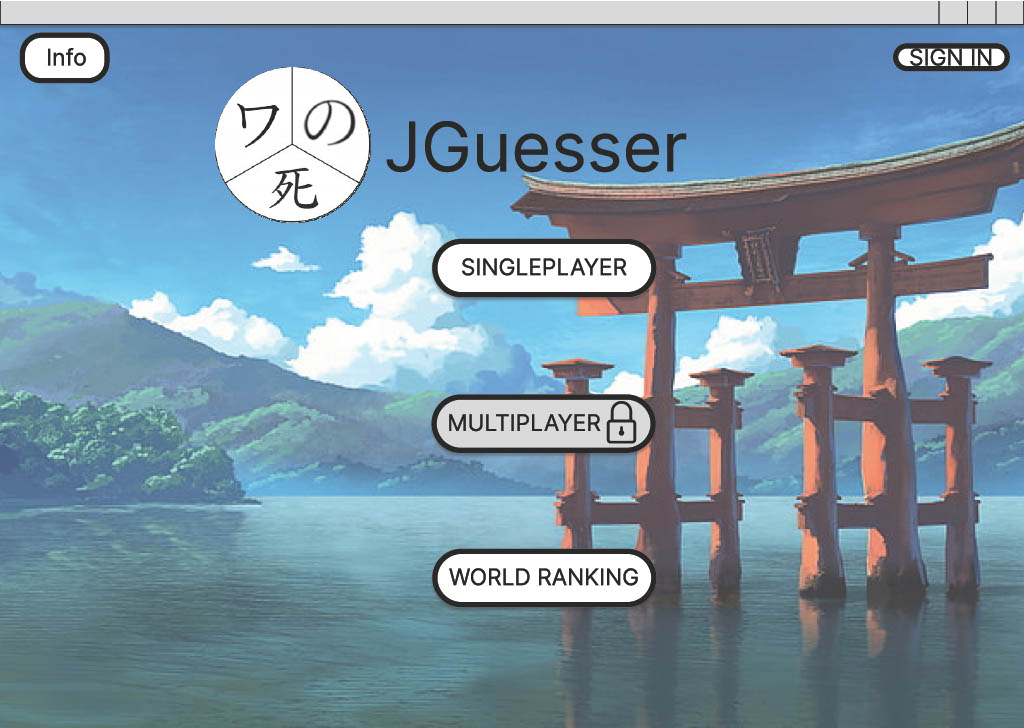
\includegraphics[scale=0.35]{images/home_page.jpg}
\end{figure}

In questa pagina sono visualizzati cinque pulsanti:
\begin{itemize}
    \item info: porta l'utente alla pagina dove potrà visualizzare gli alfabeti Hiragana, Katakana e Kanji e una breve descrizione, con relativa storia. Si fa riferimento al requisito funzionale \ref{req_compendio}.
    \item sign-in: porta l'utente alla pagina per effettuare il login. Vedere Fig:\ref{fig:schermata_login}.
    \item single-player: aprirà un'altra mini finestra, che permetterà all'utente di scegliere se giocare, con uno o più degli alfabeti a sua scelta oppure alla sfida giornaliera. Vedere Fig:\ref{fig:schermata_gioca_single-player}.
    \item multiplayer: aprirà un'altra mini finestra, che permetterà all'utente di scegliere se sfidare un giocatore a sua scelta, tramite username oppure un giocatore casuale. Vedere Fig:\ref{fig:schermata_gioca_multiplayer}.
    \item world ranking: porta l'utente alla pagina dove potrà visualizzare la classifica mondiale. Vedere Fig:\ref{fig:schermata classifica}.
\end{itemize}

\begin{figure}[!h]
\centering
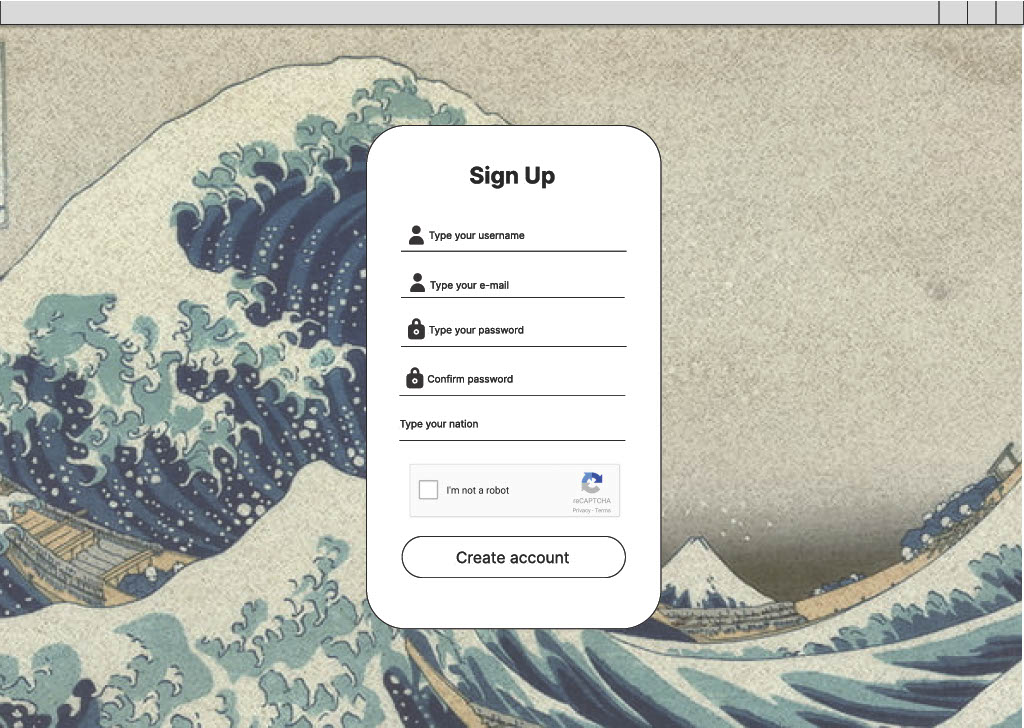
\includegraphics[scale=0.35]{images/signup.jpg}
\caption{Schermata sign-up}
\label{fig:schermata_signup}
\end{figure}
\noindent 
L'utente compila il form richiesto per registrarsi, dove dovrà inserire: e-mail, username, due volte la password e la propria nazione, dopodichè cliccando prima sul reCAPTCHA e poi sul pulsante 'create account' crea il proprio account. Si fa riferimento al requisito funzionale \ref{req_registrazione}. \\
\newpage

\begin{figure}[!h]
\centering
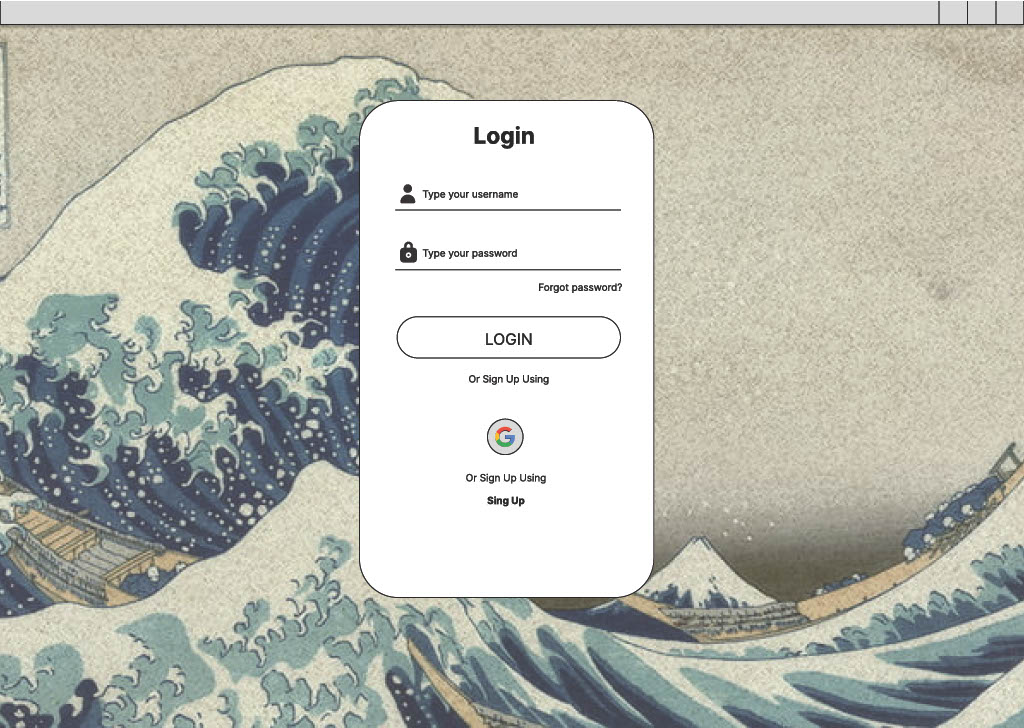
\includegraphics[scale=0.35]{images/login.jpg}
\caption{Schermata login}
\label{fig:schermata_login}
\end{figure}
\noindent 
L'utente potrà compilare il form dove dovrà inserire: username e password per accedere al proprio account, oppure nel caso non ne abbia uno avrà la possibilità di registrarsi attraverso una relativa pagina di sing-up (vedere Fig:\ref{fig:schermata_signup}). La registrazione può avvenire sia tramite l'inserimento di credenziali, ma anche utilizzando un account google. Si fa riferimento ai requisiti funzionali \ref{req_login_con credenziali} e \ref{req_login_con_google}.

\begin{figure}[!h]
\centering
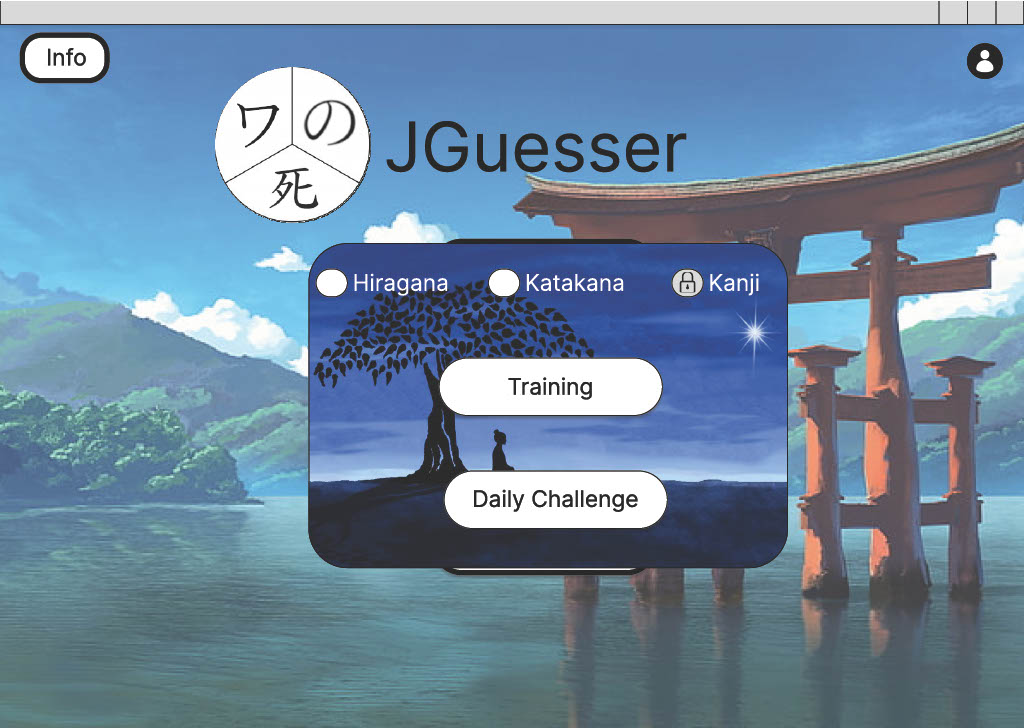
\includegraphics[scale=0.35]{images/single-player.jpg}
\caption{Schermata single-player}
\label{fig:schermata_gioca_single-player}
\end{figure}
\noindent
Questa schermata rappresenta la pagina di single-player. All'utente saranno date due possibilità. Egli potrà scegliere se allenarsi con un insieme di alfabeti a sua scelta, oppure potrà decidere di provare la sfida giornaliera. Si fa riferimento al gruppo di requisiti funzionali \ref{req_scegli_modalità_single_player}.

\begin{figure}[!h]
\centering
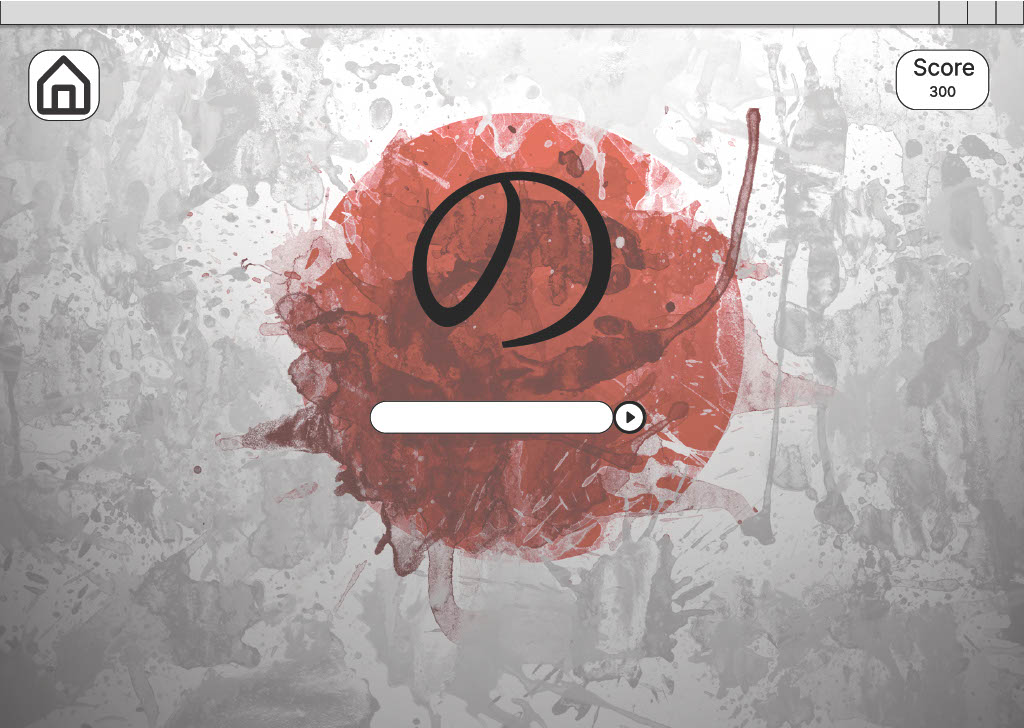
\includegraphics[scale=0.35]{images/quiz_1.jpg}
\caption{Schermata quiz tipo 1}
\label{fig:schermata_quiz_1}
\end{figure}
\noindent
Questo è come si dovrebbe presentare il quiz di tipo 1. Cliccando sul pulsante 'home' in alto a sinistra, l'utente potrà terminare la propria sessione di gioco, cliccando invece sul pulsante score l'utente potrà visualizzare una serie di statistiche temporanee. Si fa riferimento ai requisiti funzionali \ref{req_quiz_1}, \ref{req_termina_sessione_di_gioco} e \ref{req_risultato_score}.
\newpage

\begin{figure}[!h]
\centering
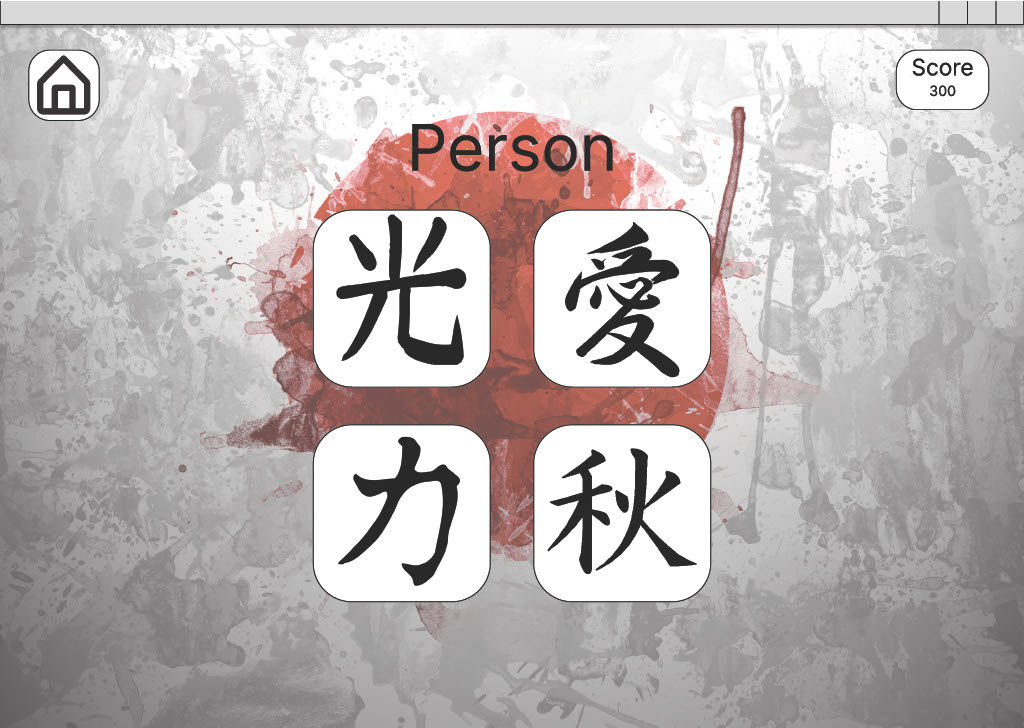
\includegraphics[scale=0.35]{images/quiz_2.jpg}
\caption{Schermata quiz tipo 2}
\label{fig:schermata_quiz_2}
\end{figure}
\noindent
Questo è come si dovrebbe presentare il quiz di tipo 2. Si fa riferimento ai requisiti funzionali \ref{req_quiz_2}, \ref{req_termina_sessione_di_gioco} e \ref{req_risultato_score}.

\begin{figure}[!h]
\centering
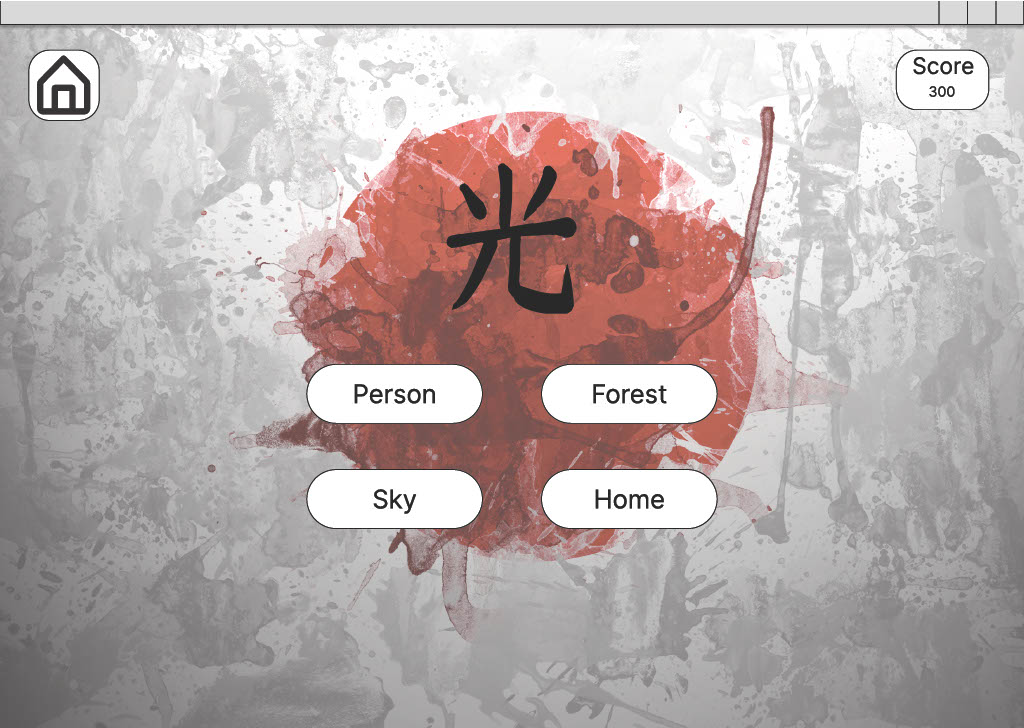
\includegraphics[scale=0.35]{images/quiz_3.jpg}
\caption{Schermata quiz tipo 3}
\label{fig:schermata_quiz_3}
\end{figure}
\noindent
Questo è come si dovrebbe presentare il quiz di tipo 3. Si fa riferimento ai requisiti funzionali \ref{req_quiz_3}, \ref{req_termina_sessione_di_gioco} e \ref{req_risultato_score}.
\newpage

\begin{figure}[!h]
\centering
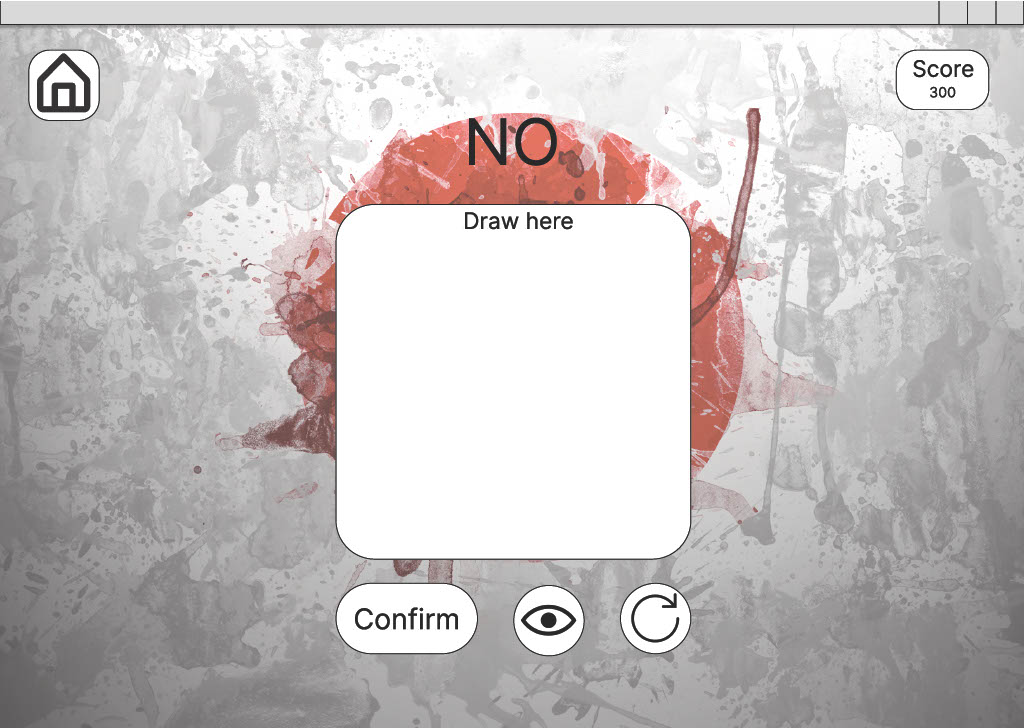
\includegraphics[scale=0.35]{images/quiz_4.jpg}
\caption{Schermata quiz tipo 4}
\label{fig:schermata_quiz_4}
\end{figure}
\noindent
Questo è come si dovrebbe presentare il quiz di tipo 4. Si fa riferimento ai requisiti funzionali \ref{req_quiz_4}, \ref{req_termina_sessione_di_gioco} e \ref{req_risultato_score}.

\begin{figure}[!h]
\centering
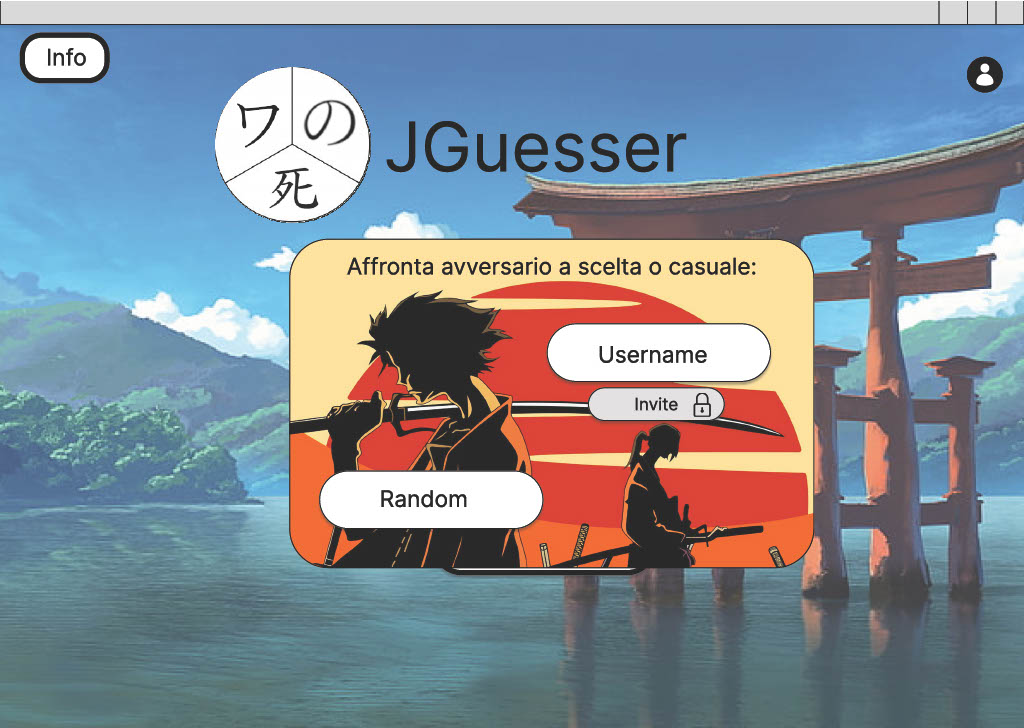
\includegraphics[scale=0.35]{images/multiplayer.jpg}
\caption{Schermata multiplayer}
\label{fig:schermata_gioca_multiplayer}
\end{figure}
\noindent
Questa schermata rappresenta la pagina di multiplayer. L'utente potrà decidere se affrontare uno specifico giocatore, inserendo il proprio username in un form e cliccando sul pulsante 'join', oppure potrà scegliere di sfidare un giocatore casuale cliccando sul pulsante 'random'. Si fa riferimento al gruppo di requsiti funzionali \ref{req_multiplayer}.

\begin{figure}[!h]
\centering
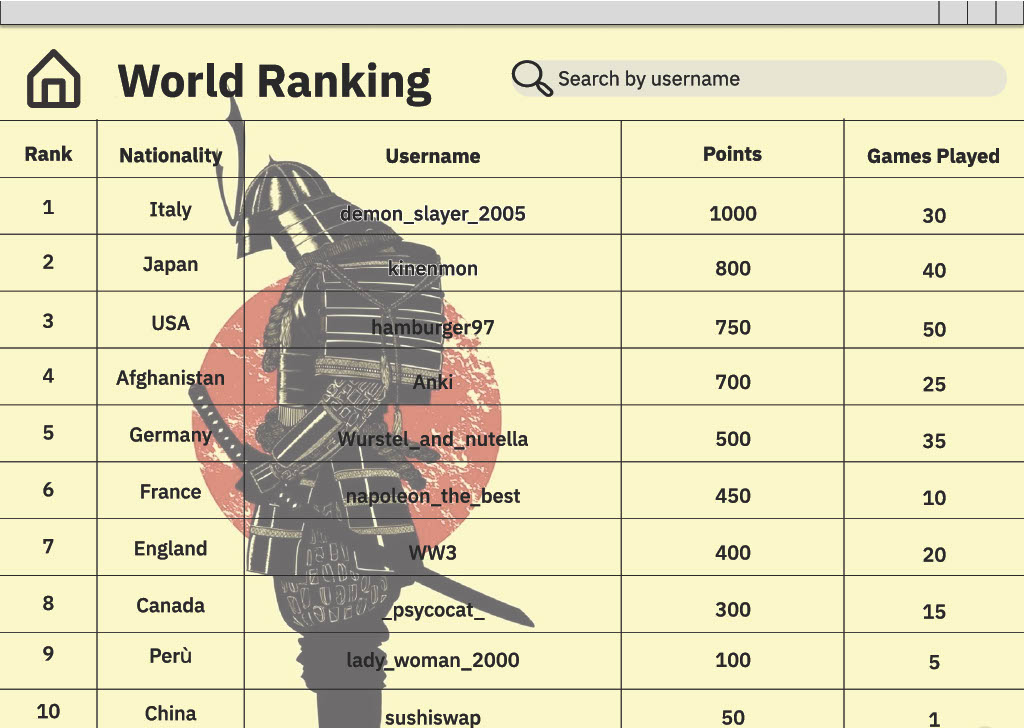
\includegraphics[scale=0.35]{images/world_ranking.jpg}
\caption{Schermata classifica}
\label{fig:schermata classifica}
\end{figure}
\noindent
Questa pagina rappresenta la classifica mondiale, che qualsiasi utente potrà visualizzare. Per ogni utente è visualizzato il proprio rank, nazionalità, username, punti (guadagnati finora) e il numero di partite giocate. L'utente potrà grazie ad una barra di ricerca, filtrare uno fra i tanti giocatori della classifica per username. Si fa riferimento ai requisiti funzionali \ref{req_visualizza_classifica} e \ref{req_ricerca_classifica}. 




\section{Design Back-end}
In questa sezione sono illustrati i sistemi esterni con il quale la nostra applicazione dovrà interagire.
\begin{figure}[!h]
\centering
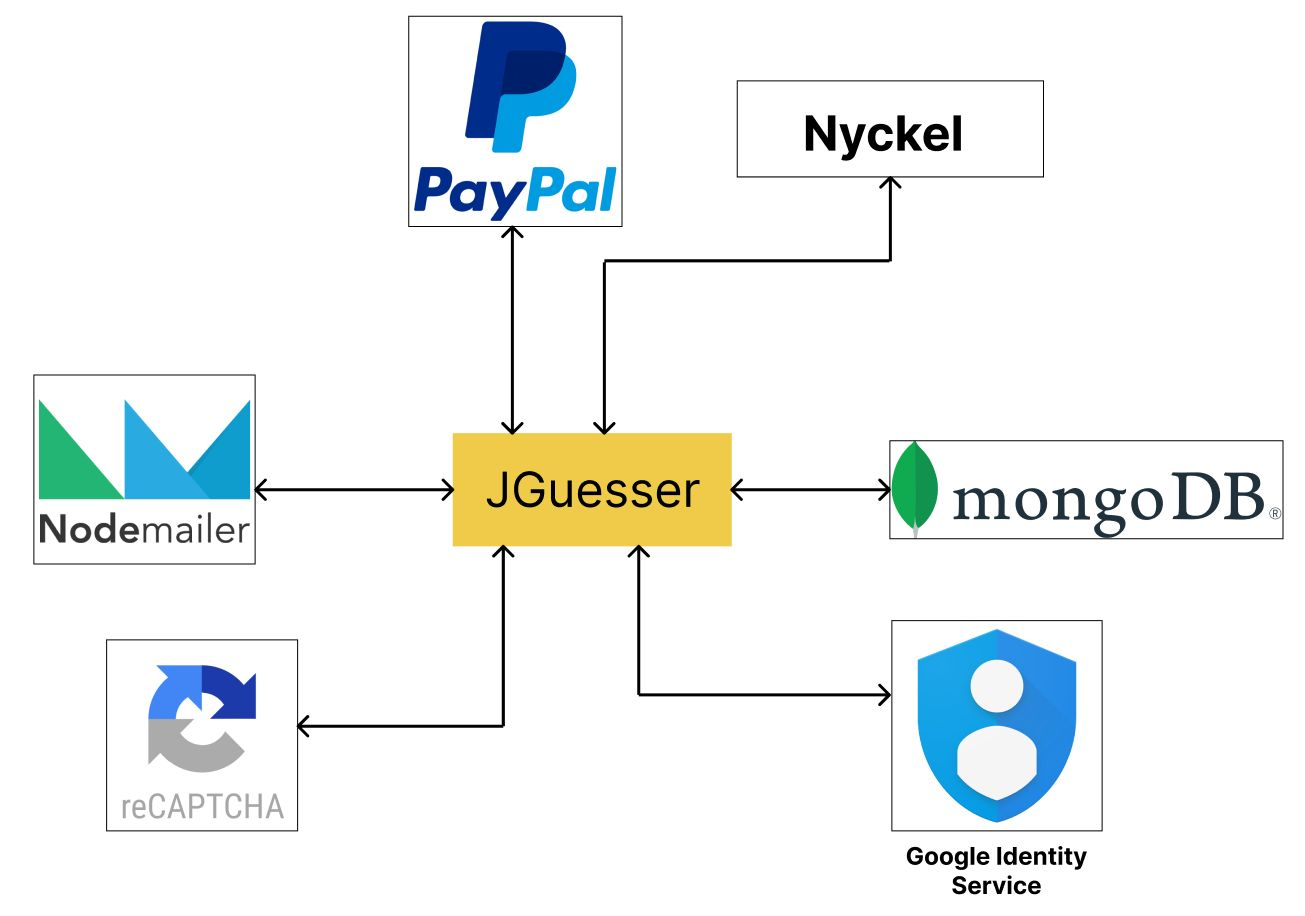
\includegraphics[scale=0.35]{images/back_end.jpg}
\caption{Schema del back-end}
\label{fig:schema_back-end}
\end{figure}

I sistemi esterni con la quale l'applicazione dovrà interfacciarsi sono i seguenti:
\begin{itemize}
    \item PayPal: sarà utilizzato come metodo di pagamento per acquistare la versione premium del servizio. L'applicazione JGuesser necessita quindi di interagire con il famoso servizio di pagamento, utilizzando le API che vengono fornite.
    \item Nyckel: machine learning API, che serviranno per classificare le immagine che l'utente disegnerà nel quiz Hiragana/Katakana di tipo 3. In questo modo il sistema sarà in grado di riconoscere se l'utente ha disegnato correttamente il simbolo relativo al suono oppure no.
    \item Nodemailer: API, che serviranno per inviare email all'utente, durante la fase di registrazione e di recupero della password, nel caso in cui egli l'abbia dimenticata.
    \item reCAPTCHA: questo servizio permette di distinguere essere umani da bot. Sarà quindi usato in fase di registrazione e recupero password, per proteggerci da spam e abusi. 
    \item Google Identity Service: questo servizio permetterà a tutti quelli utenti guest che vogliono utilizzare l'applicazione di registrarsi utilizzando un proprio account google.
    \item MongoDB: database che verrà utilizzato per memorizzare tutti i dati.
\end{itemize}

\end{document}







































































































































































%CIAO